\chapter{Implementation}
\label{chap:implementation}
%#############################################################################################

In this problem set, \textit{Kernel Ridge Regression (KRR)} and \textit{Cross-Validation (CV)} should be implemented. Section~\ref{sec:assignment1} and Section~\ref{sec:assignment2} describe the implementation of \textit{KRR} and \textit{CV}, respectively.

\section{Assignment 1: Cross-Validation}
\label{sec:assignment1}

In this assignment, \textit{Cross-Validation} should be implemented as follows:

\begin{center}
\texttt{method = cv(X, y, method, \{param\_name: value\_range, ...\}, loss\_function, nfolds, nrepetitions)}
\end{center}

The function \textit{cv} returns \textit{method}, which has been trained with the optimal parameter values. In addition, it also has an attribute \textit{method.cvloss} containing the cross validated loss.

\begin{figure}[h!]
	\centering
	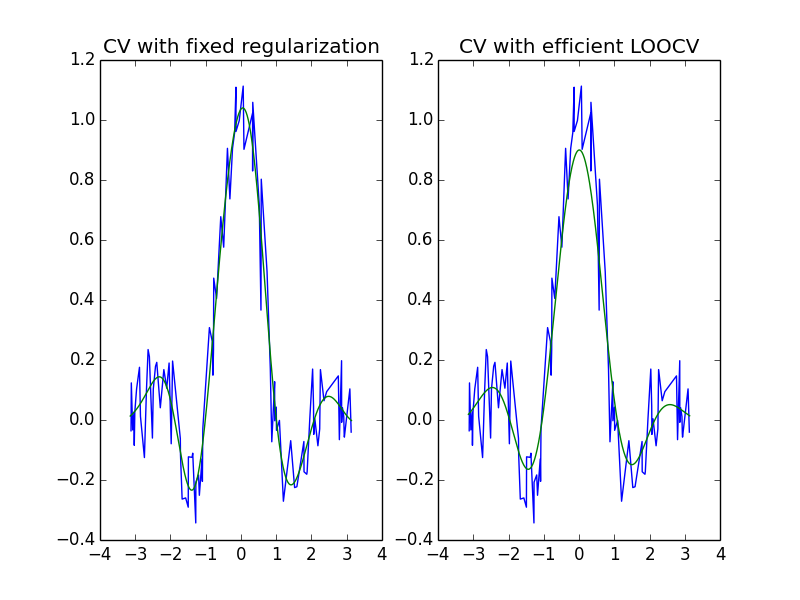
\includegraphics[scale=0.4983]{cv_test}
	\caption{CV test}
	\label{fig:cvTest}
\end{figure}

Figure~\ref{fig:cvTest} shows the test result of CV. The CV with fixed regularization took about 5.6 seconds to finish and obtained $kernelparameter=0.5994$ and $regularizationparameter=0.0774$ as the optimal parameter values. On the other hand, the CV with efficient LOOCV took about 3.3 seconds to finish and obtained $kernelparameter=0.5994$ and $regularizationparameter=1.8$ as the optimal parameter values

%######################################################################################
\section{Assignment 2: Kernel Ridge Regression}
\label{sec:assignment2}

In the second implementation assignment, \textit{Kernel-Ridge-Regression} should be implemented as a class:

\begin{center}
\texttt{class krr(X, y, kernel, kernelparameter, regularization)}
\end{center}

The \textit{krr} class has the functions \texttt{fit(X, y, kernel, kernelparameter, regularization)} and \texttt{predict(X)}. The \textit{linear}, \textit{polynomial} and \textit{gaussian} kernel should also be implemented.

\begin{figure}[h!]
	\centering
	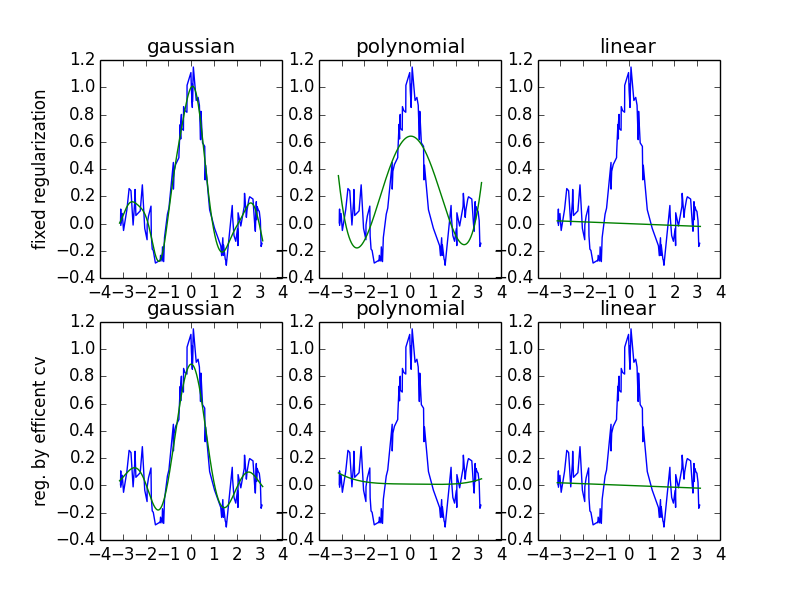
\includegraphics[scale=0.4983]{krr_test}
	\caption{KRR test}
	\label{fig:krrTest}
\end{figure}

Figure~\ref{fig:krrTest} shows the test result of \textit{krr}. The \textit{krr} was executed using fixed regularization parameter and regularization parameter obtained by efficient LOOCV. By \textit{krr} with fixed regularization parameter, the test results look promising, but by \textit{krr} with efficient LOOCV, the result of polynomial kernel did not look very good. The reason for that is i got a very high mean of the eigenvalues of the kernel, so that the regularization parameter is also very high. Maybe my polynomial kernel implementation is wrong, but i cannot find out where the mistake is. For the gaussian kernel, the regularization parameter of 1.8 was obtained, while for the polynomial and linear kernel, the regularization parameters was 1349.74 and 3.961, respectively.
